\chapter{Analysis}
\label{chap:analysis}

This chapter presents an analysis of the existing hardware. It outlines the capabilities of existing RFID/NFC readers, cloners, emulators, microcomputers, and other relevant hardware components. Specifically focusing on readers, it compares the devices based on various parameters, including compatibility with certain tag types, limitations, and pricing. Additionally, other hardware components are evaluated based on their capabilities and compatibility with RFID readers. The objective is to determine the most suitable device for integration into the portable device developed in this thesis, meeting the specified requirements effectively.


\section{Requirements}
\label{sec:requirements}

This section sets the requirements for the components of the resulting device. It describes the desired characteristics of the RFID/NFC reader, microcomputer, and its components. The resulting device composed of individual components should meet the goals specified in Chapter~\ref{chap:goals}.

\subsection{RFID/NFC Reader Requirements}

As written in Chapter~\ref{chap:theory}, there are types of tags that are easy to clone or emulate, as their main aim is to provide availability rather than integrity or confidentiality of data. In other words, some types of tags do not prioritize providing security measures. For instance, a simple 125 kHz EM410x tag holds data that can be easily read without any constraints and can be cloned or emulated quite effortlessly. Certain tags are designed to provide users with security but have failed in secure implementation. For example, their encryption algorithm has been reverse-engineered, and a variety of attacks have been published, effectively compromising their security\footnote{A perfect example of such tags are those using the encryption algorithm Crypto-1}. These tags are a little more complicated to clone, as some type of attack must be executed against the tag, exploiting its vulnerabilities. Lastly, there are tags for which no vulnerabilities or published attacks are known.

It would be beneficial to utilize an open-source reader capable of reading, writing, emulating tags, and exploiting the known vulnerabilities of some of the tags all by itself. This would help to narrow the scope of the thesis, as otherwise, the work would be very extensive. Also, the reader must be operable from the external microcomputer.

\subsection{Microcomputer Requirements}

There are various requirements for the microcomputer. One of the most crucial aspects when searching for a suitable microcomputer is its ability to communicate with the chosen reader effectively. The communication should be implementable using the chosen programming language, with minimal limitations. Another critical parameter is the ability to control the microcomputer. Most certainly, there should be a way to connect a small screen to the device. The device should be controlled via a touchscreen or connected buttons. The power consumption of the microcomputer must also be taken into account to ensure that the resulting portable device is capable of lasting a satisfying period of time.


\subsection{User Interface Requirements}

The UI of the device should meet several properties. The main characteristic may be considered the simplicity --- the device should be easy to use without any extra thinking. Another important property is the ability to enter characters. However, this, in a way, restricts the usage of physical buttons because there would have to be either too many buttons, or the entering of the characters would be too slow. This determines the direction to use a touch display instead. This way, the UI would be simple and user-friendly, without many limitations. 

The power consumption of the display is also an important evaluation criterion, and so is the size of the display, which should not be too big.


\section{Existing RFID/NFC Cloners}

This section covers various existing solutions, and devices capable of cloning or emulating tags. It provides a general overview of their capabilities, prices, and potential limitations.

\subsection{Flipper Zero}

The Flipper Zero is one of the most well-known gadgets. Among its capabilities, such as emulating a BadUSB device\footnote{A so-called BadUSB device is a device that is recognized by computers as a human interface device, such as a keyboard~\cite{badusb}.} or controlling devices that utilize radio signals below 1 GHz, it can also operate at frequencies of 125 kHz and 13.56 MHz for RFID tags~\cite{flipper}. It offers a highly portable solution for reading, writing, cloning, and emulating tags, supporting various types, such as MIFARE Classic 1k or MIFARE Ultralight~\cite{flipperreading}.  Its software is licensed under GPL-3.0, making it fully modifiable and distributable under the same license~\cite{githubflipper}.

The device is powered by an integrated lithium-ion polymer rechargeable battery, with power management efficiently handled to provide operation for up to a month without recharging.~\cite{flipperpower}

However, a significant drawback is the fact that this device is already a completely standalone unit. The device is available for purchase on the official website for 165 Euros~\cite{flippershop}. Although this price may seem high, it is essential to consider that the device offers significantly more functionalities than those outlined in Section~\ref{sec:requirements}.


\subsection{Chameleon Mini}

The Chameleon Mini is a versatile credit-card shaped RFID and NFC tool, often used for security compliance, analysis, penetration testing, and various applications. Its fully open-source platform supports emulating perfect clones of various commercial smartcards, including the UID and even cryptographic functions. Its human-readable command set provides users the ability to configure settings and content for up to 8 internally stored virtual cards. Integrated buttons and LEDs enable user interaction while in standalone mode, meaning when the device is not connected to the computer.~\cite{chameleonwiki}

Despite its capability to read and emulate various types of high frequency cards, its firmware does not provide the ability to write cards. To crack cards, the device itself supports only a MFKey32 attack, where the attacker has to have also an access to the reader itself to catch and decode transmitted keys. This does not quite meet our requirements. ~\cite{lab401chameleon}

Its battery life is quite extensive, it contains a Li-ion battery which is capable of running the device for up to 1 year with an average usage of 15 seconds a day. The device is quite expensive, it can be purchased for around 130 Euros.~\cite{lab401chameleon}

This powerful and highly modifiable device supports the emulation of cards of various types, however, its software cannot write cards.


\subsection{Chameleon Ultra}

Chameleon Ultra is a relative of Chameleon Mini, one of the smallest solutions in existence. It's about the size of a keychain, capable of reading, emulating, writing, and even cracking tags. It boasts better emulation capabilities than Flipper Zero, but also than Proxmark.~\cite{chameleonultra}

It is controlled via CLI and GUI interfaces, but can also be controlled via a mobile app. Includes a 90 mAh LiPo battery that lasts up to a month without a charge.~\cite{chameleonultra}

Its huge disadvantage is its price. The device is available for 155 euros~\cite{chameleonultra}. The huge advantage is its capabilities in comparison, if we think about the size of the device.

This device meets all the requirements, but the decision must take into account its price. 


\subsection{NXP PN532 Module}

The NXP PN532 is a highly integrated module operating at 13.56 MHz frequencies. It supports 6 different operating modes,
\begin{itemize}
    \item ISO/IEC 14443A/MIFARE Reader/Writer,
    \item FeliCa Reader/Writer,
    \item ISO/IEC 14443B Reader/Writer,
    \item ISO/IEC 14443A/MIFARE Card MIFARE Classic 1K or MIFARE Classic 4K card emulation mode,
    \item FeliCa Card emulation, and
    \item ISO/IEC 18092, ECMA 340 Peer-to-Peer.~\cite{pn532doc}
\end{itemize}

With various libraries, it is possible to perform for example an offline nested attack~\cite{nestedpn532} or a darkside attack~\cite{darksidepn532} in the computer. However, these attacks are not done in the module itself, but in the connected computer.

Another library makes possible to write Gen 3 Magic MIFARE Classic tags and Gen 2 Magic MIFARE Classic tags.~\cite{clonerpn532}

It can be classified as an affordable device, a man can buy this device for only around 10 Euros.~\cite{pn532shop}

This device can be controlled via Arduino microcontroller, however, its downside is the restriction to 13.56 MHz frequencies.


\subsection{Proxmark}

The Proxmark is an RFID tool, supporting vast majority of RFID tags worldwide. It allows both low level and high level interactions with the tags. It is adapted to many industries and users, its possibilities are used by people from the academic research, product development or penetration testing.~\cite{proxmark}

Its functionalities include the ability to read tags, write tags, write magic tags, simulate tags, and even crack the tags, meaning the Proxmark software includes attacks against various known tags vulnerabilities. \cite{proxmarkwiki}

There are a number of variants of the Proxmark on the market, including cheap clones, which however can be flashed with the software and are supported.~\cite{proxmarkclones}

The device can be connected to a computer with an USB cable and it is controlled via a command-line interface~\cite{proxmarkcommands}. It also supports a standalone mode, which is a mode, in which the device can be utilized without connection to the computer. However, the standalone mode is quite limiting, because the device itself contains only one simple button and LED indicators - this does not allow more complicated user input.~\cite{proxmarkstandalone}

The price of one of the cheaper variants of the Proxmark, the Proxmark 3 Easy, is around 75 Euros~\cite{proxmarkshop}.


\section{Existing Microcomputers}

This section covers various existing microcomputers. Provides a general overview of the capabilities, and options for connecting other modules, such as displays or the reader itself.


\subsection{Arduino}

Arduino is an open-source platform featuring easy to use hardware boards, containing a microcontroller, and input/output pins for connecting all kinds of peripherals. It is programmable by \emph{Arduino programming language}, which is based on \emph{Wiring}\footnote{\emph{Wiring} is an open-source programming framework for microcontrollers~\cite{wiring}.}.~\cite{arduino}

There are available many types of Arduino boards, that vary in size, number of pins or computing power.~\cite{arduinohardware} Also, there are available many Arduino accessories, including various types of screens, buttons, or even RFID/NFC readers\footnote{As an example could be used the aforementioned PN532 module.}. 

It is still safe to say that the price of the boards is quite low, even more when Arduino clones\footnote{These clones are cheaper unofficial versions of the original Arduino boards.} are taken to consideration.


\subsection{Raspberry Pi}

Raspberry Pi produces a series of single-board modular microcomputers that are built on the Arm architecture and also Raspberry Pi Pico boards for lower-power and real-time applications. The series of microcomputers run the Linux operating system, which makes them exceptionally potent for a diverse number of tasks. Every Raspberry Pi board is backed by extensive technical documentation, and enthusiastic community.~\cite{raspberry}

Each board has several input/output pins, number of models contain also RJ45 network ports, USB ports, or even HDMI ports.

Similar to the Arduino, the Raspberry Pi has many modules available, including screens, for which there are open-source drivers and libraries available.

The price of a Raspberry Pi 4 model B, containing all the ports mentioned previously, goes from 35 Euros~\cite{raspberryshop}.


\section{Comparison}

For clarity, following tables give an overview of the properties of all components. This will help to select the most suitable ones.

\subsection{Comparison of Readers}

\begin{table}[h]
    \caption[Readers comparison]{~Comparison of tag readers}\label{tab:readers}
    \centering
    \renewcommand{\arraystretch}{1.3}
    \begin{tabularx}{\textwidth}{@{}l *7{|>{\centering\arraybackslash}X}}
    Device &  LF & HF & Read & Crack & Write magic & Emulate & Price \\ \hline \hline
    Flipper Zero & \faCheck & \faCheck & \faCheck & \faCheck & \faCheck & \faCheck & High \\ \hline
    ChameleonMini & ~ & \faCheck & \faCheck & ~ & ~ & \faCheck & High \\ \hline
    ChameleonUltra & \faCheck & \faCheck & \faCheck & \faCheck & \faCheck & \faCheck & High \\ \hline
    PN532 module & ~ & \faCheck & \faCheck & ~ & \faCheck & \faCheck & Low \\ \hline
    Proxmark & \faCheck & \faCheck & \faCheck & \faCheck & \faCheck & \faCheck & Middle \\ 
    \end{tabularx}
\end{table}

The Table~\ref{tab:readers} shows a comparison of the mentioned RFID/NFC tag readers. Only Proxmark and Chameleon Ultra meet the specified requirements, as the other readers mentioned lack important features, such as low-frequency card support for the NIX PN532 module and Chameleon Mini. The Flipper Zero does not meet our requirements as it is already a standalone unit --- the Flipper Zero could not be used as a component in the final device.

The Chameleon Ultra ticks all the boxes, but is very expensive for the purposes of this thesis. In contrast, the price of Proxmark is satisfactory because it is far from the highest and still meets all the conditions.

The big advantage of Proxmark is a great support --- the Github repository containing the device firmware and also the desktop client is regularly updated. A disadvantage may be the size of the device, the Proxmark 3 Easy type has dimensions of 54 mm × 86.6 mm~\cite{dimensionsproxmark}. However, this might not matter so much, it will also depend on the size of the microcomputer selected. 

Since the Proxmark is the most capable of the devices analyzed and the price is acceptable, this device is chosen as the reader used for this project.


\subsection{Comparison of Microcomputers}

\begin{table}[h]
    \caption[Microcomputers comparison]{~Comparison of microcomputers}\label{tab:microcomputers}
    \centering
    \renewcommand{\arraystretch}{1.3}
    \begin{tabularx}{\textwidth}{@{}l *5{|>{\centering\arraybackslash}X}}
    Device &  Easy communication with Proxmark & Energy consumption & Touch display available & Capabilities & Price \\ \hline \hline
    Arduino & ~ & Low~\cite{arduinodoc} & \faCheck & Low & Low \\ \hline
    Raspberry Pi & \faCheck & High~\cite{raspberrydoc} & \faCheck & High & Low \\
    
    \end{tabularx}
\end{table}

The Table~\ref{tab:microcomputers} shows a comparison of the mentioned microcomputers. Both options are strong candidates, but implementing Arduino communication with Proxmark would be much more challenging than providing Raspberry Pi communication via USB port. 

In terms of extensibility, again, both are very good, but the Raspberry Pi is slightly better. With the computational power of the Raspberry Pi, other types of attacks could be implemented in the future, with the computations taking place within the microcomputer itself. The Raspberry itself has Bluetooth and Wi-Fi support built in by default, and in the future it would be much easier to control the device via, for example, a mobile phone than it would be with an Arduino.

Likewise, implementing a software user interface will be much easier on the Raspberry Pi, as it runs Linux and thus has many graphical programming language libraries to choose from.  

The disadvantages of the Raspberry Pi may be its size and power consumption, which is high compared to the Arduino. 


\section{Conclusion of the Analysis}

Several RFID/NFC reader solutions were analysed, and it was found that many of them could function as standalone units. After careful consideration of the requirements, Proxmark was selected as the most suitable reader for our project. Additionally, the Raspberry Pi was identified as the most appropriate microcomputer for this work.

After analyzing the different types of Proxmark, the Proxmark 3 Easy was selected. It is one of the cheapest variants of Proxmark and at the same time it is not deprived of any important functionality.

After analyzing the different types of Raspberry Pi, the Raspberry Pi 4 B variant with 4 GB of RAM was selected. This variant is one of the newer and more powerful ones. However, it is also quite large, but this does not matter because the selected Proxmark 3 Easy is almost the same size and therefore choosing a smaller microcomputer would not reduce the overall size of the resulting device.

The Waveshare 3.5" LCD touchscreen is suitable as a display for the device, which is the same size as the Raspberry Pi and Proxmark. It is connected and powered via 26 pins. There are freely available drivers to make it easily usable.~\cite{waveshare35inch}

\begin{figure}[h]
    \centering
    \begin{minipage}[b]{0.45\textwidth}
        \centering
        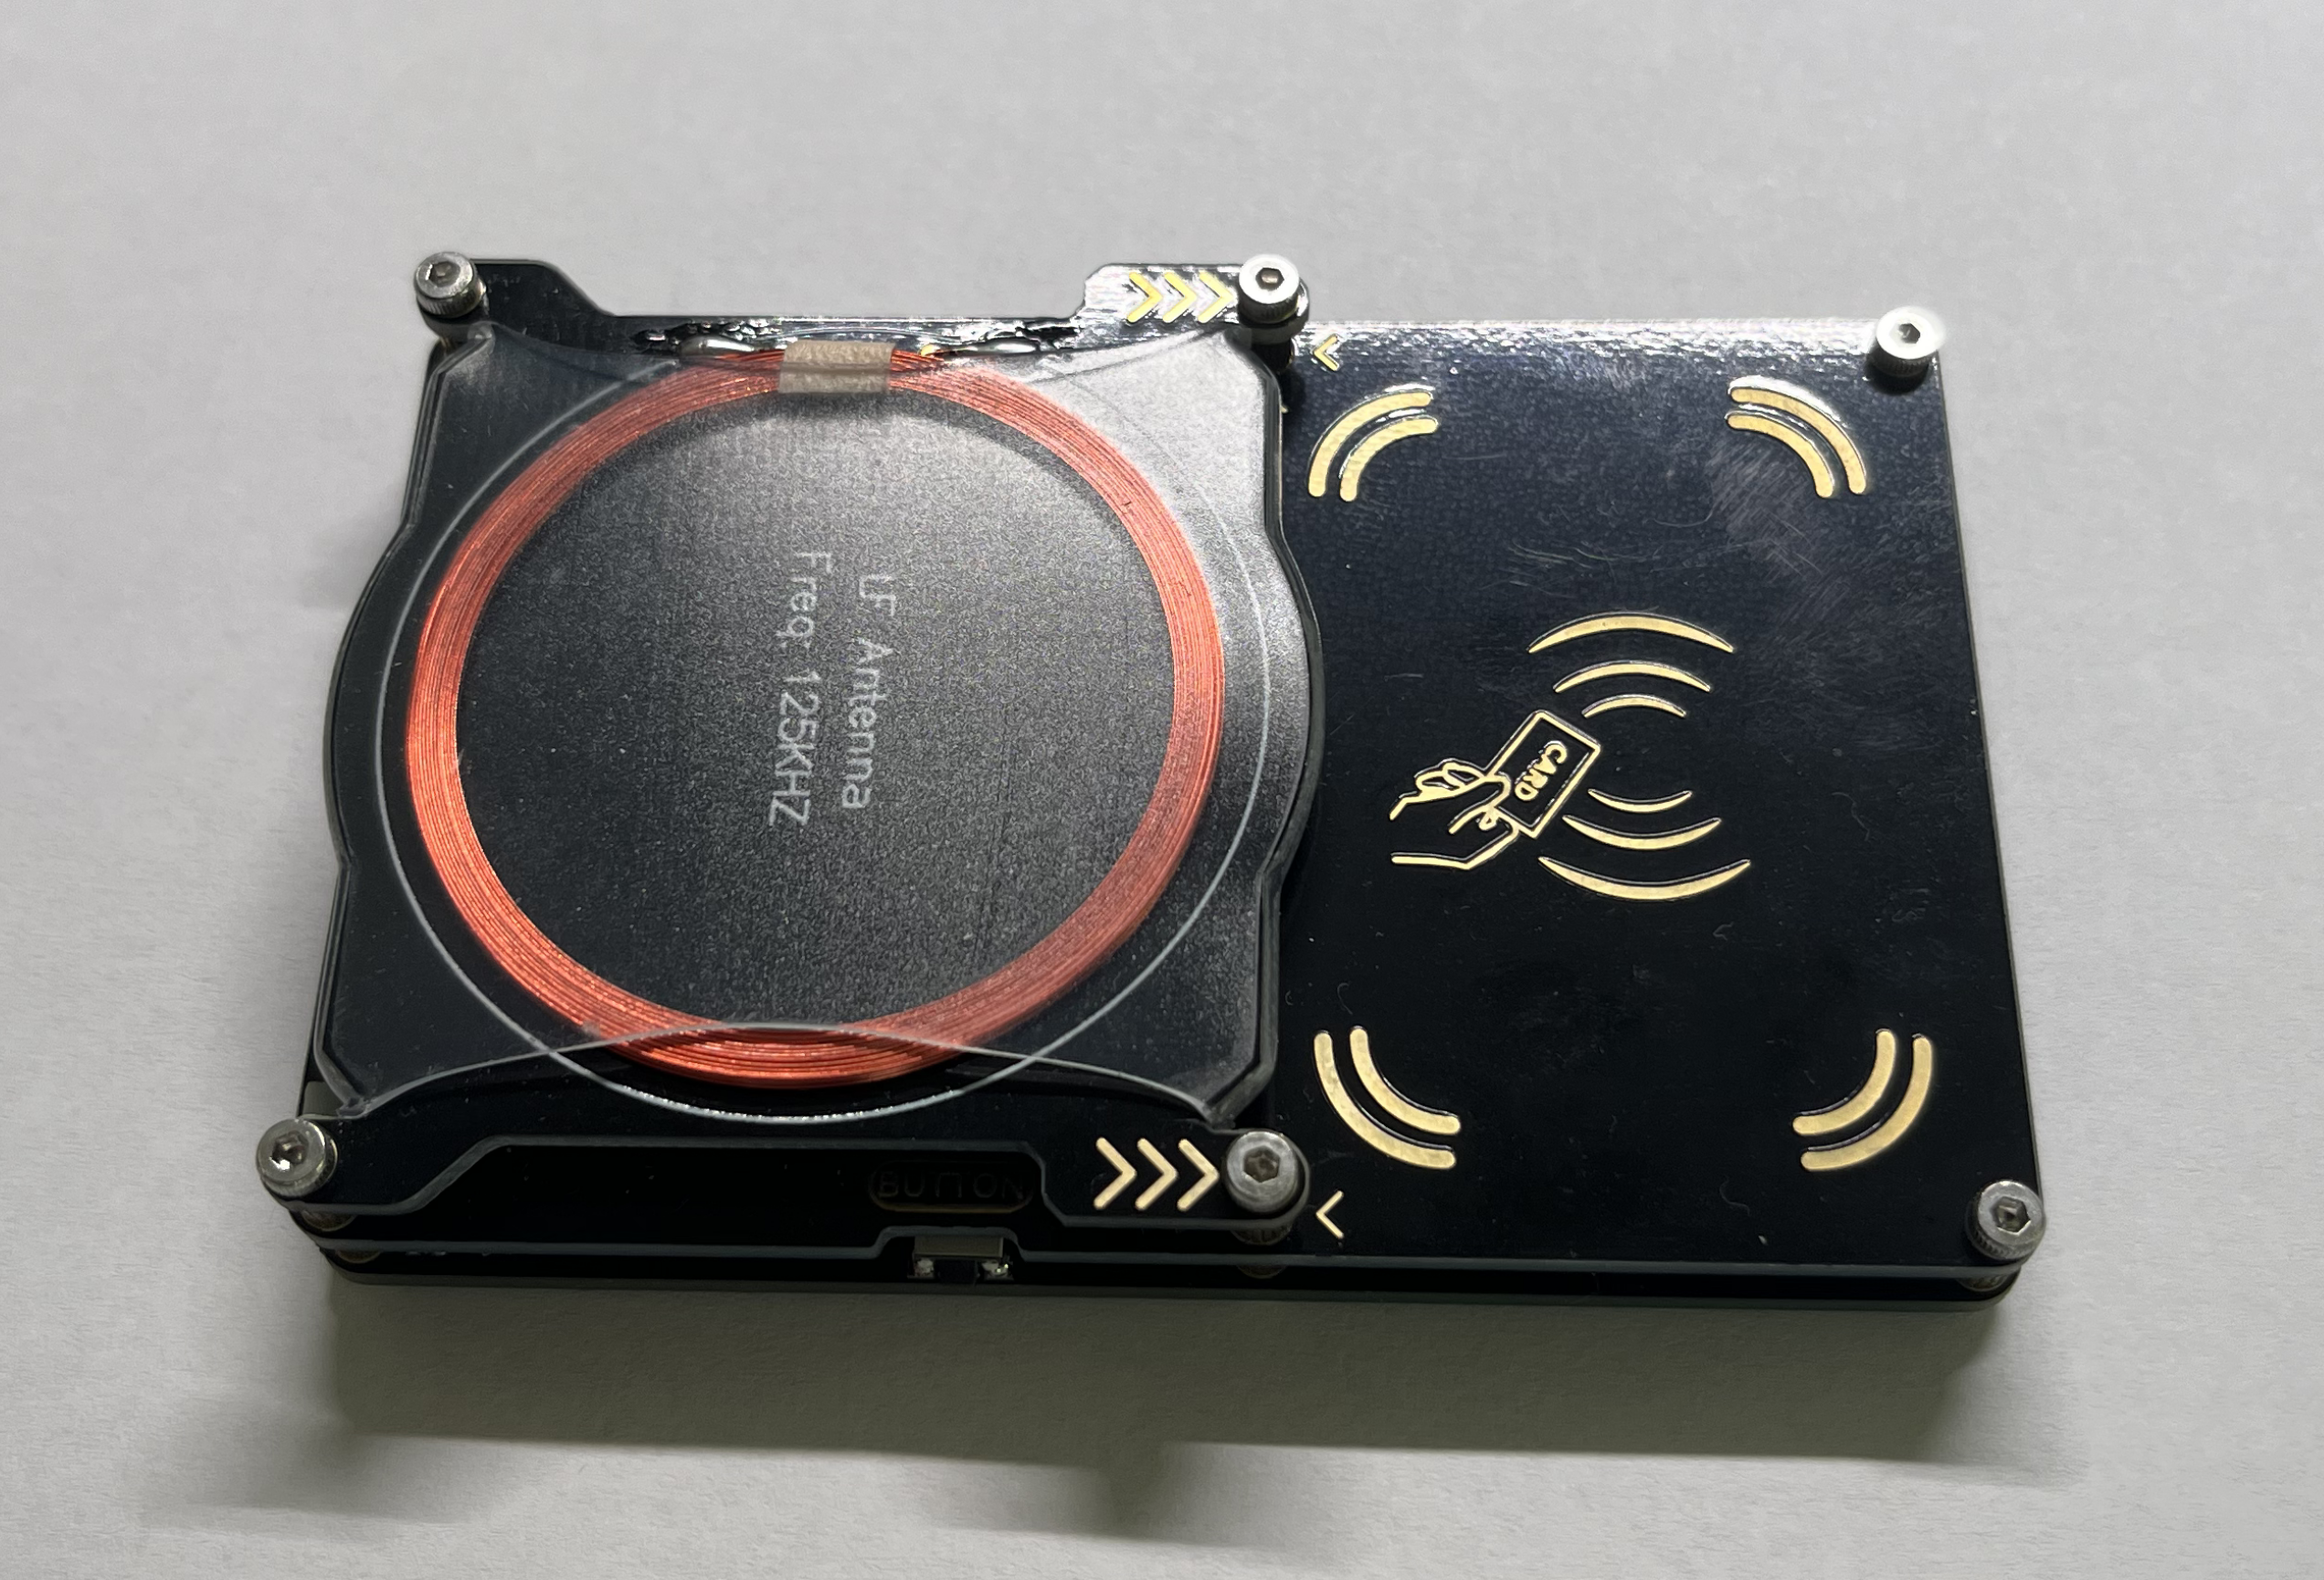
\includegraphics[width=\textwidth]{text/proxmark.png}
        \caption{~Photo of Proxmark 3 Easy}
        \label{fig:sub1}
    \end{minipage}
    \hfill
    \begin{minipage}[b]{0.45\textwidth}
        \centering
        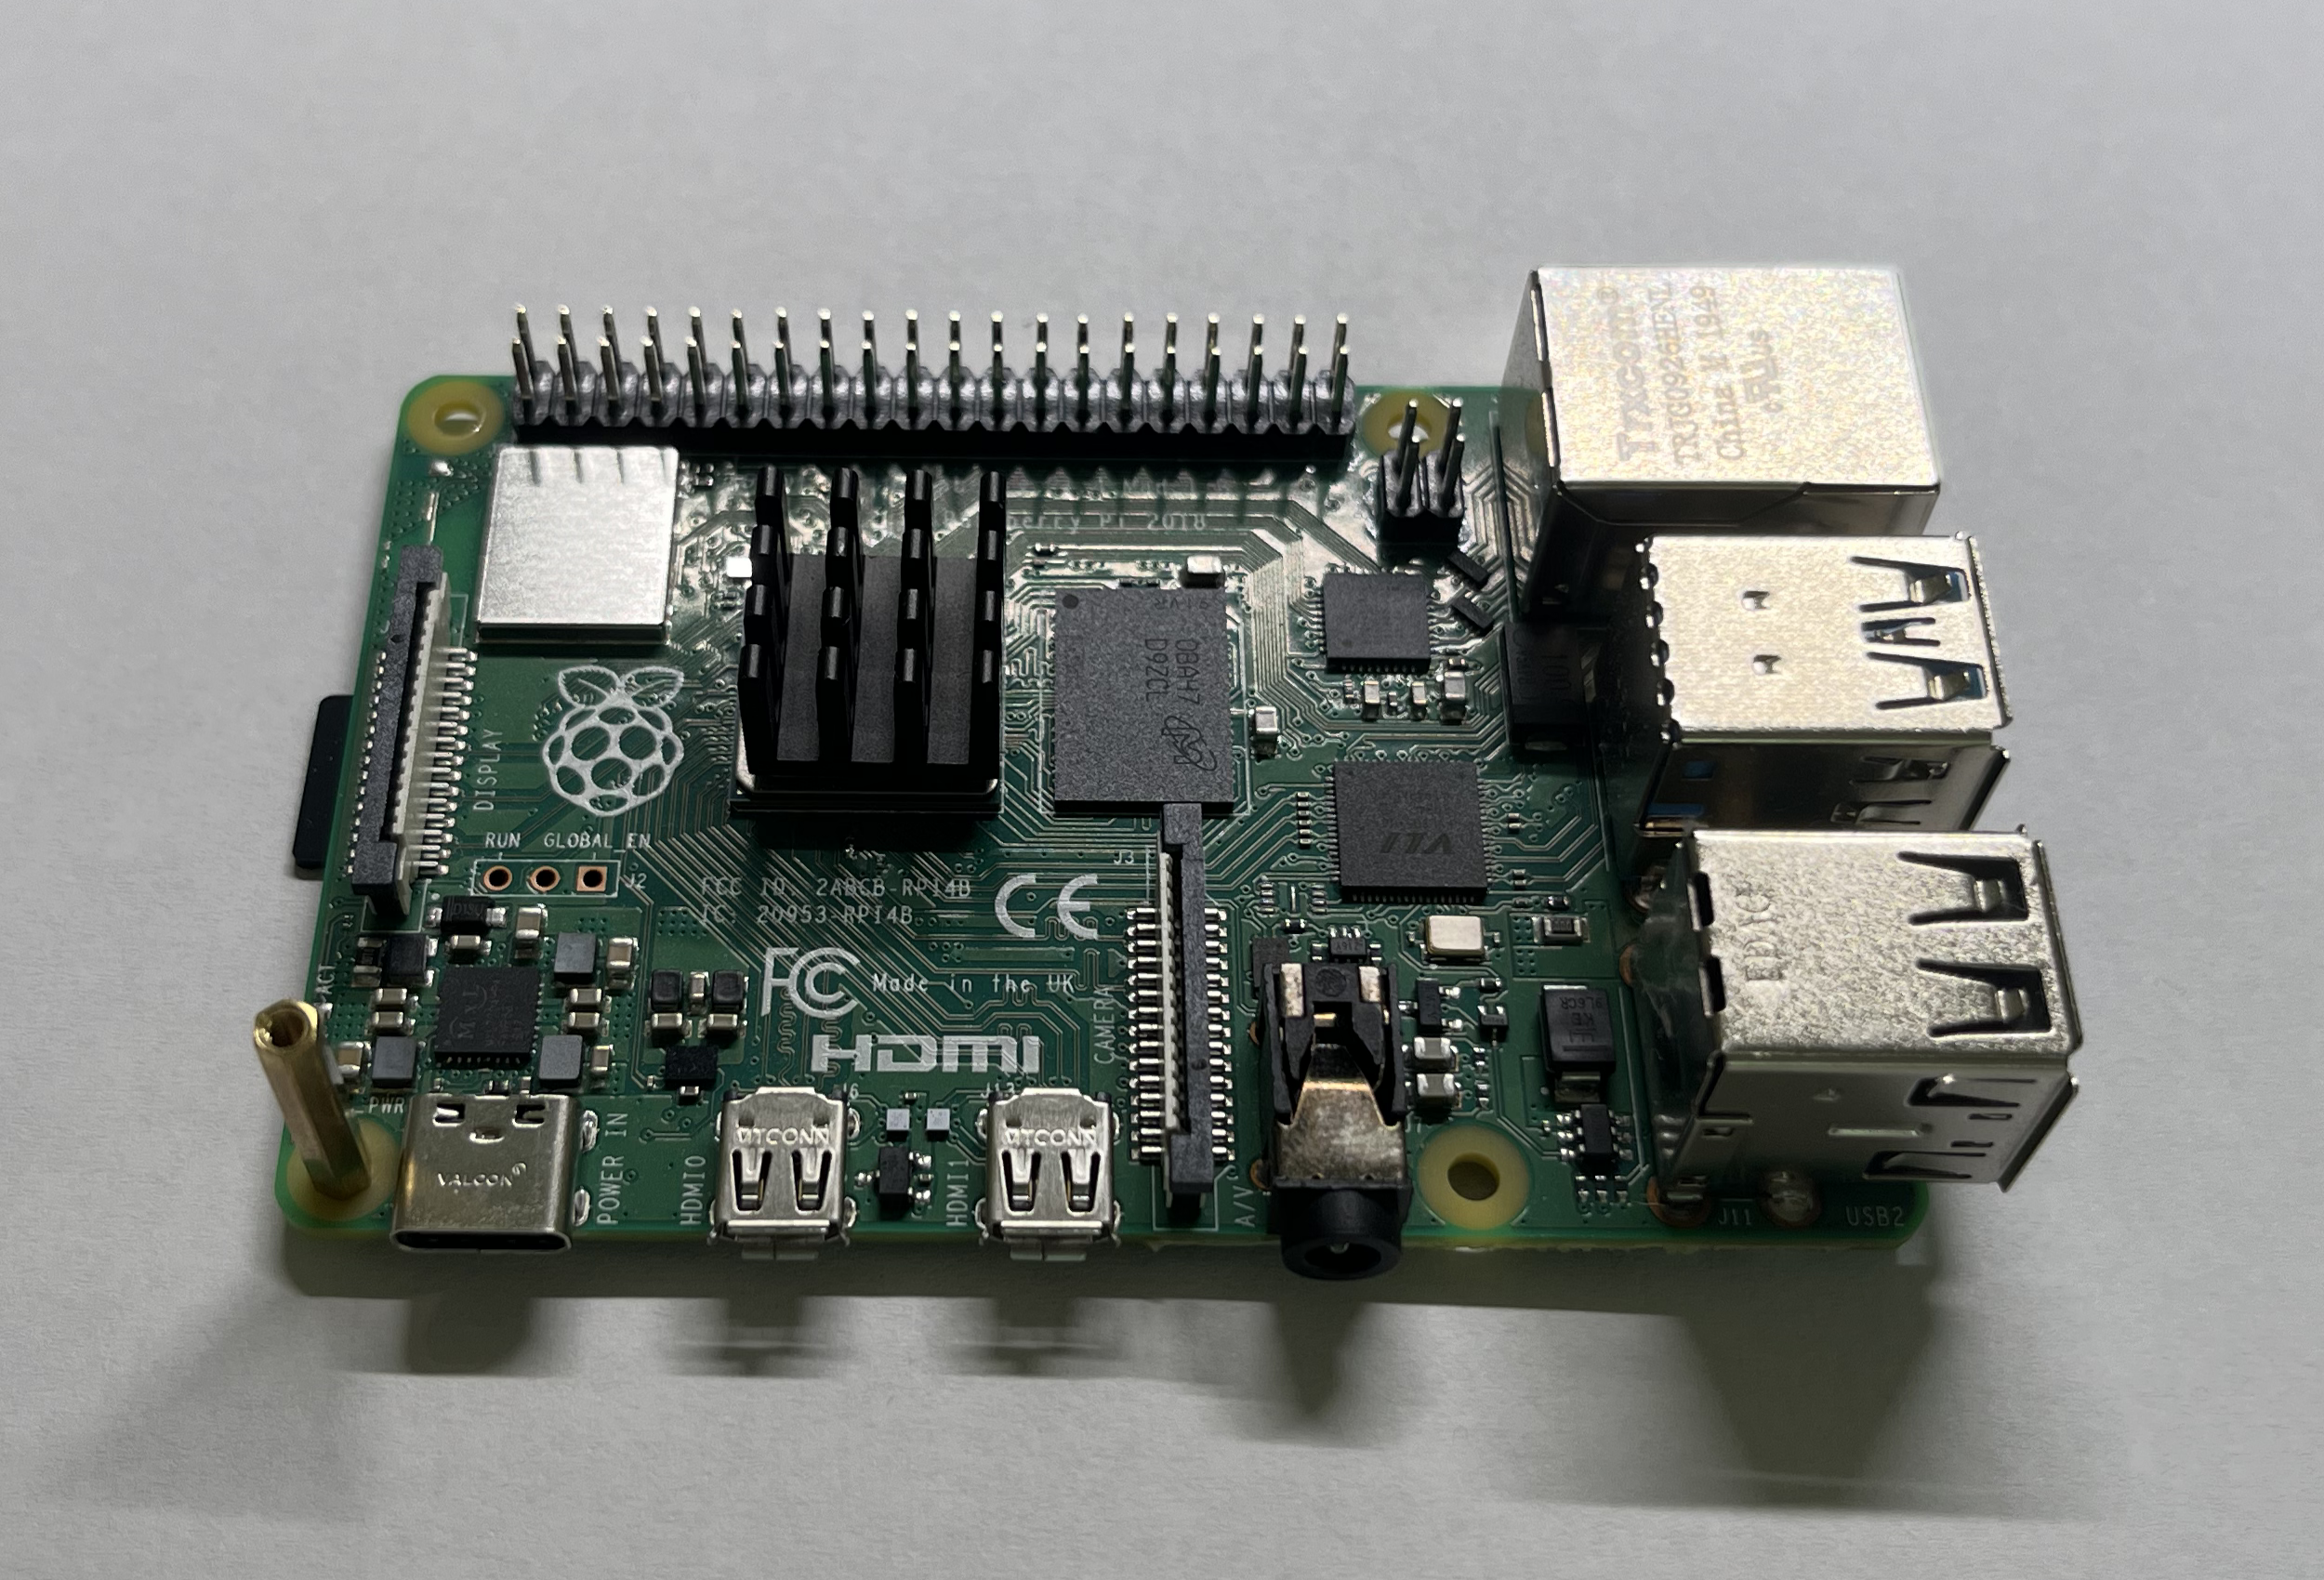
\includegraphics[width=\textwidth]{text/raspberry.png}
        \caption{~Photo of Raspberry Pi 4 B}
        \label{fig:sub2}
    \end{minipage}
    \label{fig:main}
\end{figure}